\documentclass[12pt, a4paper]{article}

% Required packages
\usepackage{amsmath}        % For advanced math environments
\usepackage{amssymb}        % For math symbols
\usepackage{geometry}       % For setting page margins
\usepackage{pgfplots}       % For creating plots
\usepackage{siunitx}        % For typesetting units
\usepackage[hidelinks]{hyperref} % For hyperlinks (optional)

% Tikz libraries for arrows and styling
\usetikzlibrary{arrows.meta, decorations.markings}

% PGFPlots settings
\pgfplotsset{compat=1.17}   % Use a recent compatibility version

% Custom TikZ style for arrows on plots
\tikzset{
  arrow_style/.style={
    decoration={
      markings,
      mark=at position #1 with {\arrow{Stealth[scale=1.5]}}
    },
    postaction={decorate}
  }
}

% Set page geometry
\geometry{a4paper, margin=1in}

% Title
\title{Notes and Problems on Thermodynamic PV Processes}
\author{A Review for Calculations}
\date{\today}

\begin{document}

\maketitle
\tableofcontents
\newpage

\section{Key Concepts and Equations}

\subsection{Fundamentals \& The First Law of Thermodynamics}
In thermodynamics, we study a \textbf{system} (e.g., a gas in a cylinder) and its interaction with the \textbf{surroundings}. The total energy contained within the system is its \textbf{internal energy ($U$)}.

Energy can be transferred in two ways:
\begin{itemize}
    \item \textbf{Heat (Q):} Energy transfer due to a temperature difference. \textbf{$Q$ is positive} when heat flows \textit{into} the system.
    \item \textbf{Work (W):} Energy transfer via mechanical means. \textbf{$W$ is positive} when work is done \textit{on} the system (i.e., it contracts).
\end{itemize}

These are linked by the \textbf{First Law of Thermodynamics}, a statement of energy conservation:
$$ \Delta U = Q + W $$
The increase in a system's internal energy ($\Delta U$) equals the heat added to it ($Q$) plus the work done on it ($W$).

For an \textbf{ideal gas}, the internal energy is a function of temperature only:
$$ \Delta U = nC_V \Delta T $$
where $n$ is the number of moles and $C_V$ is the molar heat capacity at constant volume. The work done by an expanding or contracting gas corresponds to the area under its path on a Pressure-Volume (P-V) diagram.

\subsection{The Four Key Processes}

\subsubsection{1. Isobaric Process (Constant Pressure)}
An isobaric process occurs at a constant pressure ($\Delta P = 0$). Imagine heating a gas in a cylinder with a piston that is free to move.
\begin{center}
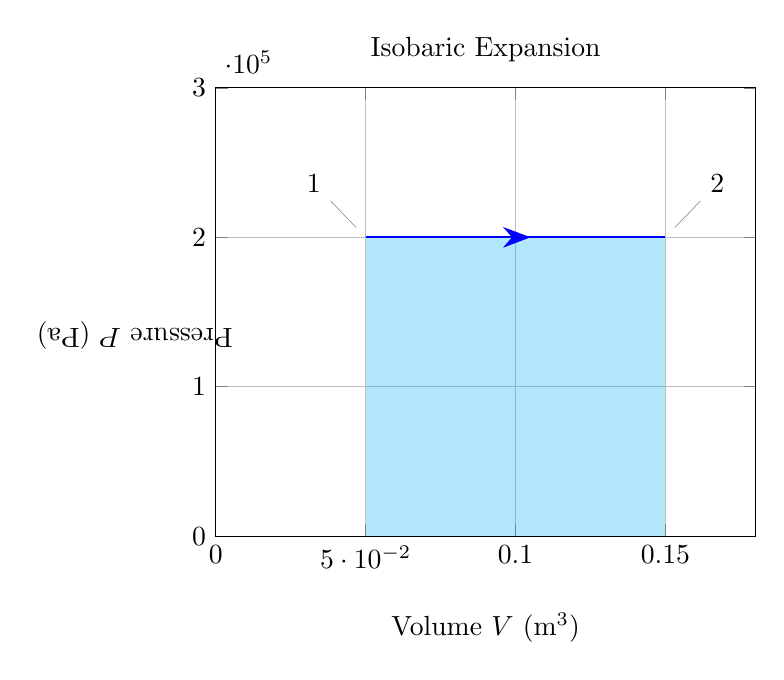
\begin{tikzpicture}
    \begin{axis}[
        title={Isobaric Expansion},
        xlabel={Volume $V$ (\si{m^3})}, ylabel={Pressure $P$ (\si{Pa})},
        xlabel style={at={(axis description cs:0.5,-0.15)},anchor=north},
        ylabel style={at={(axis description cs:-0.15,0.5)},anchor=south,rotate=90},
        xmin=0, xmax=0.18, ymin=0, ymax=3e5, grid=major,
    ]
    \addplot [fill=cyan, opacity=0.3, draw=none] coordinates {(0.05, 0) (0.05, 2e5) (0.15, 2e5) (0.15, 0)};
    \addplot [thick, blue, arrow_style=0.55] coordinates {(0.05, 2e5) (0.15, 2e5)};
    \node[pin=135:{$1$}] at (axis cs:0.05, 2e5) {};
    \node[pin=45:{$2$}] at (axis cs:0.15, 2e5) {};
    \end{axis}
\end{tikzpicture}
\end{center}
\textbf{Key Equations:}
\begin{itemize}
    \item \textbf{Work Done (W):} $W = -P \Delta V = -P(V_2 - V_1)$
    \item \textbf{Heat (Q):} $Q = nC_P \Delta T$
    \item \textbf{Internal Energy ($\Delta U$):} $\Delta U = nC_V \Delta T$
\end{itemize}
\textbf{Illustration:} See Problem 1, where a gas expands at $2 \times 10^5$ Pa. The work done on gas, $W = -(2 \times 10^5) \times (0.15 - 0.05) = -20,000$ J, is the rectangular area under the graph.

\subsubsection{2. Isochoric Process (Constant Volume)}
An isochoric process occurs at a constant volume ($\Delta V = 0$), such as in a rigid, sealed container. Since the volume cannot change, the gas cannot do any work.
\begin{center}
\begin{tikzpicture}
    \begin{axis}[
        title={Isochoric Heating},
        xlabel={Volume $V$ (\si{m^3})}, ylabel={Pressure $P$ (\si{Pa})},
        xlabel style={at={(axis description cs:0.5,-0.15)},anchor=north},
        ylabel style={at={(axis description cs:-0.15,0.5)},anchor=south,rotate=90},
        xmin=0, xmax=0.012, ymin=0, ymax=3.5e5, xtick={0, 0.008314}, xticklabels={$0$, $V_0$}, grid=major,
    ]
    \addplot [thick, green!60!black, arrow_style=0.55] coordinates {(0.008314, 1.5e5) (0.008314, 3e5)};
    \node[pin=180:{$1$}] at (axis cs:0.008314, 1.5e5) {};
    \node[pin=180:{$2$}] at (axis cs:0.008314, 3e5) {};
    \end{axis}
\end{tikzpicture}
\end{center}
\textbf{Key Equations:}
\begin{itemize}
    \item \textbf{Work Done (W):} $W = 0$
    \item \textbf{First Law Simplification:} $\Delta U = Q$
    \item \textbf{Heat (Q):} $Q = nC_V \Delta T$
\end{itemize}
\textbf{Illustration:} See Problem 4. Since the container is rigid, $W = 0$. All heat added goes directly into increasing the internal energy.

\subsubsection{3. Isothermal Process (Constant Temperature)}
An isothermal process occurs at a constant temperature ($\Delta T = 0$). To keep the temperature constant during a compression or expansion, heat must be transferred.
\begin{center}
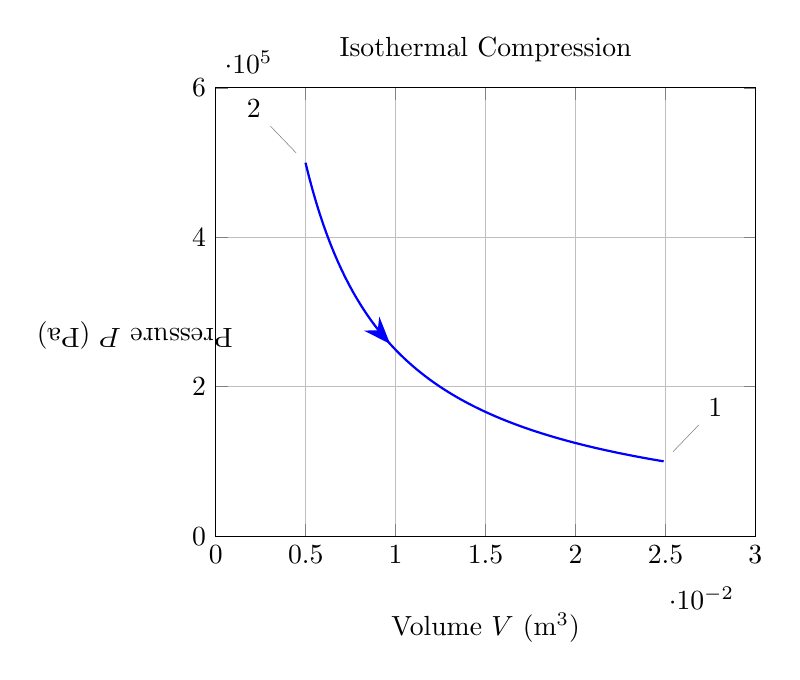
\begin{tikzpicture}
    \begin{axis}[
        title={Isothermal Compression},
        xlabel={Volume $V$ (\si{m^3})}, ylabel={Pressure $P$ (\si{Pa})},
        xlabel style={at={(axis description cs:0.5,-0.15)},anchor=north},
        ylabel style={at={(axis description cs:-0.15,0.5)},anchor=south,rotate=90},
        xmin=0, xmax=0.03, ymin=0, ymax=6e5, grid=major,
    ]
    \addplot [domain=0.00499:0.0249, samples=100, thick, blue, arrow_style=0.4] {2494.2/x};
    \node[pin=45:{$1$}] at (axis cs:0.0249, 1e5) {};
    \node[pin=135:{$2$}] at (axis cs:0.00499, 5e5) {};
    \end{axis}
\end{tikzpicture}
\end{center}
\textbf{Key Equations:}
\begin{itemize}
    \item \textbf{Internal Energy ($\Delta U$):} $\Delta U = 0$
    \item \textbf{First Law Simplification:} $Q = W$
    \item \textbf{Work Done by gas (W):} $W = nRT \ln\left(\frac{V_2}{V_1}\right) = nRT \ln\left(\frac{P_1}{P_2}\right)$
\end{itemize}
\textbf{Illustration:} See Problem 2. To compress the gas without its temperature rising, heat must be removed. Thus, $Q=W \approx -4014$ J.

\subsubsection{4. Adiabatic Process (No Heat Exchange)}
An adiabatic process occurs with no heat exchange ($Q = 0$). This happens in a perfectly insulated system or a process that is very rapid.
\begin{center}
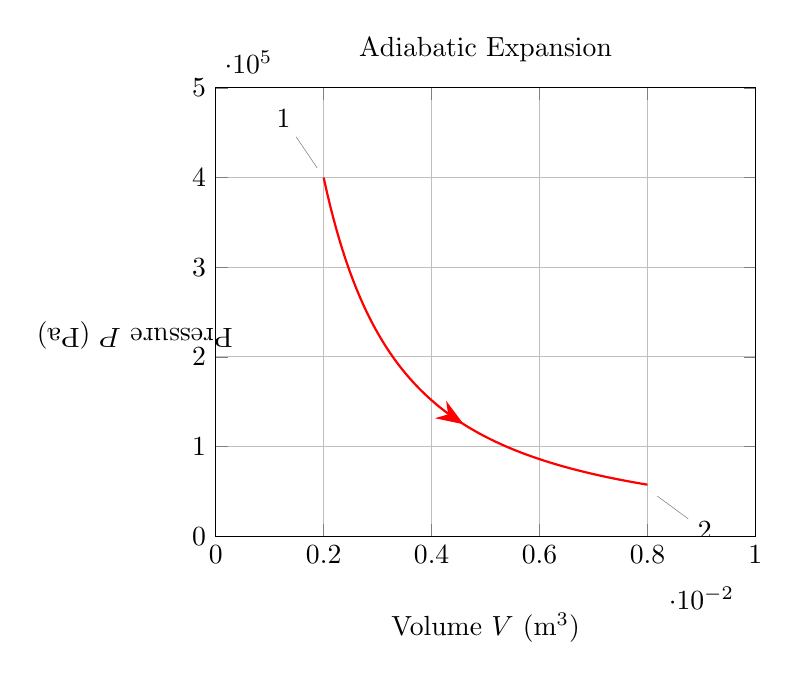
\begin{tikzpicture}
    \begin{axis}[
        title={Adiabatic Expansion},
        xlabel={Volume $V$ (\si{m^3})}, ylabel={Pressure $P$ (\si{Pa})},
        xlabel style={at={(axis description cs:0.5,-0.15)},anchor=north},
        ylabel style={at={(axis description cs:-0.15,0.5)},anchor=south,rotate=90},
        xmin=0, xmax=0.01, ymin=0, ymax=5e5, grid=major,
        ]
    \addplot [domain=0.002:0.008, samples=100, thick, red, arrow_style=0.6] {66.59/(x^1.4)};
    \node[pin=120:{$1$}] at (axis cs:0.002, 4e5) {};
    \node[pin=-30:{$2$}] at (axis cs:0.008, 5.28e4) {};
    \end{axis}
\end{tikzpicture}
\end{center}
\textbf{Key Equations:}
\begin{itemize}
    \item \textbf{Heat (Q):} $Q = 0$
    \item \textbf{First Law Simplification:} $\Delta U = -W$
    \item \textbf{Process Relationship:} $P_1 V_1^\gamma = P_2 V_2^\gamma$, where $\gamma = C_P/C_V$.
    \item \textbf{Work Done by gas(W):} $W = \frac{P_1V_1 - P_2V_2}{\gamma - 1}$
\end{itemize}
\textbf{Illustration:} See Problem 3. As the gas expands and does work, its energy must come from its own internal energy, causing it to cool down.

\subsection{Cyclic Processes}
A cyclic process is a series of processes that returns the system to its initial state.
\begin{itemize}
    \item \textbf{Internal Energy:} Over a full cycle, the net change is zero: $\Delta U_{cycle} = 0$.
    \item \textbf{Net Work ($W_{net}$):} From the First Law, $W_{net} = Q_{net}$.
    \item \textbf{P-V Diagram:} The net work done is the \textbf{area enclosed by the loop}.
    \item \textbf{Engine Efficiency ($\eta$):} The ratio of net work output to heat input.
    $$ \eta = \frac{W_{net}}{Q_{in}} $$
\end{itemize}

\newpage
\section{Illustrative Problems}

\subsection{Problem 1: Isobaric Expansion}
\subsubsection*{Problem Statement}
A cylinder fitted with a frictionless piston contains 2 moles of an ideal diatomic gas at an initial volume of $V_1 = 0.05 \, \text{m}^3$ and a pressure of $P = 2 \times 10^5 \, \text{Pa}$. The gas is heated and expands at constant pressure to a final volume of $V_2 = 0.15 \, \text{m}^3$.
Calculate: 1. Work done ($W$), 2. Change in internal energy ($\Delta U$), 3. Heat supplied ($Q$). (Use $C_V = \frac{5}{2}R$)

\subsubsection*{Solution}
\paragraph{1. Work Done ($W$)}
$W = P \Delta V = (2 \times 10^5 \, \text{Pa}) \times (0.15 - 0.05 \, \text{m}^3) = \mathbf{20,000 \, J}$
\paragraph{2. Change in Internal Energy ($\Delta U$)}
$T_1 = \frac{PV_1}{nR} \approx 601.4 \, \text{K}$ and $T_2 = \frac{PV_2}{nR} \approx 1804.2 \, \text{K}$.
$\Delta U = n C_V \Delta T = (2) \left(\frac{5}{2} R\right) (1804.2 - 601.4) \approx \mathbf{50,000 \, J}$
\paragraph{3. Heat Supplied ($Q$)}
$Q = \Delta U + W = 50,000 \, \text{J} + 20,000 \, \text{J} = \mathbf{70,000 \, J}$

\subsection{Problem 2: Isothermal Compression}
\subsubsection*{Problem Statement}
One mole of an ideal monatomic gas is compressed isothermally at $T = 300 \, \text{K}$ from $P_1 = 1 \times 10^5 \, \text{Pa}$ to $P_2 = 5 \times 10^5 \, \text{Pa}$.
Calculate: 1. Work done ($W$), 2. Change in internal energy ($\Delta U$), 3. Heat transferred ($Q$).
\subsubsection*{Solution}
\paragraph{1. Work Done ($W$)}
$W = nRT \ln\left(\frac{P_1}{P_2}\right) = (1)(8.314)(300) \ln\left(\frac{1}{5}\right) \approx \mathbf{-4014 \, J}$
\paragraph{2. Change in Internal Energy ($\Delta U$)} Since $\Delta T = 0$, $\mathbf{\Delta U = 0}$.
\paragraph{3. Heat Transferred ($Q$)} From the First Law, $Q = W \approx \mathbf{-4014 \, J}$.

\subsection{Problem 3: Adiabatic Expansion}
\subsubsection*{Problem Statement}
An ideal diatomic gas ($\gamma = 1.4$) at $P_1 = 4 \times 10^5 \, \text{Pa}$, $V_1 = 2 \, \text{L}$ expands adiabatically to $V_2 = 8 \, \text{L}$. Calculate: 1. Final pressure ($P_2$), 2. Work done ($W$).
\subsubsection*{Solution}
\paragraph{1. Final Pressure ($P_2$)}
$P_2 = P_1 \left(\frac{V_1}{V_2}\right)^\gamma = (4 \times 10^5) \left(\frac{2}{8}\right)^{1.4} \approx \mathbf{5.28 \times 10^4 \, Pa}$
\paragraph{2. Work Done ($W$)}
$W = \frac{P_1 V_1 - P_2 V_2}{\gamma - 1} = \frac{(4 \times 10^5)(0.002) - (5.28 \times 10^4)(0.008)}{1.4 - 1} = \mathbf{944 \, J}$

\subsection{Problem 4: Isochoric Heating}
\subsubsection*{Problem Statement}
$0.5$ moles of ideal gas at $P_1 = 1.5 \times 10^5 \, \text{Pa}$, $T_1 = 300 \, \text{K}$ is heated at constant volume until $P_2 = 3.0 \times 10^5 \, \text{Pa}$. Calculate: 1. Work ($W$), 2. Final temperature ($T_2$), 3. Heat added ($Q$) for a monatomic gas ($C_V = \frac{3}{2}R$).
\subsubsection*{Solution}
\paragraph{1. Work Done ($W$)} Since $\Delta V = 0$, $\mathbf{W = 0}$.
\paragraph{2. Final Temperature ($T_2$)} $T_2 = T_1 \left(\frac{P_2}{P_1}\right) = 300 \, \text{K} \times 2 = \mathbf{600 \, K}$.
\paragraph{3. Heat Added ($Q$)} $Q=\Delta U = n C_V \Delta T = (0.5) \left(\frac{3}{2} R\right) (300) \approx \mathbf{1871 \, J}$.

\subsection{Problem 5: A Four-Process Thermodynamic Cycle}
\subsubsection*{Problem Statement}
One mole of a monatomic ideal gas ($\gamma=5/3$) undergoes the cycle A $\to$ B $\to$ C $\to$ D $\to$ A.
\begin{itemize}
    \item State A: $P_A = 1 \times 10^5 \, \text{Pa}$, $V_A = 0.02 \, \text{m}^3$.
    \item A $\to$ B: Isobaric expansion to $V_B = 0.04 \, \text{m}^3$.
    \item B $\to$ C: Isothermal expansion to $V_C = 0.06 \, \text{m}^3$.
    \item C $\to$ D: Isochoric cooling.
    \item D $\to$ A: Adiabatic compression.
\end{itemize}
Calculate the net work done ($W_{net}$) and the thermal efficiency ($\eta$).
\subsubsection*{Solution}
\paragraph{1. Find state variables}
A: ($10^5$ Pa, $0.02$ m$^3$). B: ($10^5$ Pa, $0.04$ m$^3$). C: ($0.667 \times 10^5$ Pa, $0.06$ m$^3$). D: ($0.192 \times 10^5$ Pa, $0.06$ m$^3$).
\paragraph{2. Work and Heat}
$W_{AB} = 2000$ J. $Q_{AB} \approx 5000$ J (in).
$W_{BC} \approx 1622$ J. $Q_{BC} \approx 1622$ J (in).
$W_{CD} = 0$. (Heat out).
$W_{DA} \approx -1272$ J. $Q_{DA} = 0$.
\paragraph{3. Net Work and Efficiency}
$W_{net} = W_{AB} + W_{BC} + W_{CD} + W_{DA} \approx \mathbf{2350 \, J}$.
$Q_{in} = Q_{AB} + Q_{BC} \approx \mathbf{6622 \, J}$.
$\eta = \frac{W_{net}}{Q_{in}} = \frac{2350}{6622} \approx 0.355 \quad \text{or} \quad \mathbf{35.5\%}$.
\begin{center}
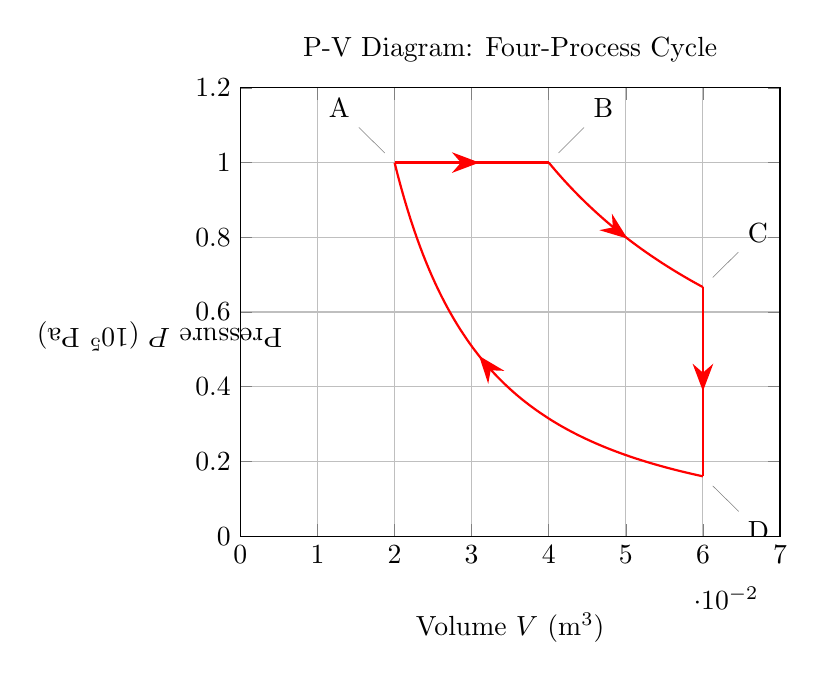
\begin{tikzpicture}
    \begin{axis}[
        title={P-V Diagram: Four-Process Cycle},
        xlabel={Volume $V$ (\si{m^3})}, ylabel={Pressure $P$ ($10^5$ \si{Pa})},
        xlabel style={at={(axis description cs:0.5,-0.15)},anchor=north},
        ylabel style={at={(axis description cs:-0.15,0.5)},anchor=south,rotate=90},
        xmin=0, xmax=0.07, ymin=0, ymax=1.2,
        yticklabel style={/pgf/number format/fixed}, grid=major,
    ]
    % Define coordinates for precision
    \pgfmathsetmacro{\PA}{1} \pgfmathsetmacro{\VA}{0.02}
    \pgfmathsetmacro{\PB}{\PA} \pgfmathsetmacro{\VB}{0.04}
    \pgfmathsetmacro{\VC}{0.06} \pgfmathsetmacro{\PC}{\PB*\VB/\VC}
    \pgfmathsetmacro{\VD}{\VC} \pgfmathsetmacro{\GAMMA}{5/3}
    \pgfmathsetmacro{\PD}{\PA*(\VA/\VD)^\GAMMA}

    % Draw paths using the defined coordinates for a perfect loop
    \addplot [thick, red, arrow_style=0.55] coordinates {(\VA, \PA) (\VB, \PB)}; % A->B
    \addplot [thick, red, arrow_style=0.55, domain=\VB:\VC, samples=50] {(\PB*\VB)/x}; % B->C
    \addplot [thick, red, arrow_style=0.55] coordinates {(\VC, \PC) (\VD, \PD)}; % C->D
    \addplot [thick, red, arrow_style=0.55, domain=\VD:\VA, samples=100] {(\PA*(\VA^\GAMMA))/(x^\GAMMA)}; % D->A

    % Annotations
    \node[pin=135:{A}] at (axis cs:\VA, \PA) {};
    \node[pin=45:{B}] at (axis cs:\VB, \PB) {};
    \node[pin=45:{C}] at (axis cs:\VC, \PC) {};
    \node[pin=-45:{D}] at (axis cs:\VD, \PD) {};
    \end{axis}
\end{tikzpicture}
\end{center}

\end{document}